\documentclass[9pt,twocolumn,twoside]{styles/osajnl}
\usepackage{fancyvrb}
\journal{i524} 

\title{Nagios - Example Paper for I524}

\author[1]{Tony Liu}
\author[1]{Vibhatha Abeykoon}
\author[1]{Gregor von Laszewski}

\affil[1]{School of Informatics and Computing, Bloomington, IN 47408, U.S.A.}


\dates{paper-1, \today}

\ociscodes{Cloud, I524}

% replace this with your url in github/gitlab
\doi{\url{https://github.com/vibhatha/sp17-i524/blob/master/paper1/S17-TS-0003/report.pdf}}


\begin{abstract}
Nagios is a platform/tool, which provides a set of software for system and network infrastructure monitoring. Within this article, we explored what problem it tried to solve, how it solved the problem, and why it's important to have Nagios. We took a close look at the main components of Nagios and how it works.
\end{abstract}

\setboolean{displaycopyright}{true}

\begin{document}

\maketitle

\section{Introduction}

According to ~\cite{nagios-book}, even through the machines have become more and 
more critical to us human being, yet they are untrustworthy. We couldn't agree more with the author on this. The newest example on this is the GitLab.com incident happened on Jan 31st 2017. A tired system administrator, working late at night in the Netherlands, had accidentally deleted a directory on the wrong server during a frustrating database replication process: he wiped a folder containing 300GB of live production data that was due to be replicated~\cite{gitlabmeltdown}. Mistakes could be corrected easily since Gitlab have deployed several methods to backup and replicate the production data and all they just need to do is to recover and restore from the backup. However, after several attempts, they found that out of 5 backup/replication techniques deployed none were working reliably or set up in the first place. People haven't emphasize enough about how crucial it is to backup the important data. However, none of this matters if the backup mechanism no long works. That is the exact reason why we explore Nagios in this paper.


\section{What is Nagios}

Nagios ~\cite{www-nagios, wiki-nagios} is a system, network and infrastructure monitoring tool under open source license that provides instant awareness of mission-critical IT infrastructure. Nagios allows to monitor the infrastructure, alert the system admin, provide visualized reports, schedule downtime for maintenance, and plan upgrade in advance with trends and capacity diagrams. Its design emphasizes highly on flexibility and scalability. To provide such flexibility, Nagios is composed of different modules. The reason behind this modular design is that Nagios fully considers the variety of systems and networks it will monitor on. Different customers require a large amount of customization before they themselves know they do.

\subsection{Architecture}

As in ~\cite{nagios-paper-2012}, let's take a look at how Nagios works in a network monitoring system. Since Nagios has a flexible modular architecture, it allows user to customize modules to adapt the network it monitors on. 

The main component is Nagios core, which is a scheduler daemon detecting network devices and services regularly. The core will alert administer by several notification methods like email, message and web interface. 

Nagios plugin is an executable that takes arguments to trigger some actions and print results. It has two types, check and notification. Both are used by Nagios core. The check plugin is used to check and monitor devices and services. The notification plugin is used to send out alerts if the check plugin detected any status change. Beside these two, the users themselves can develop their own custom plugins. 

Nagios module is a procedure that calls upon API called Nagios Event Broker. The user could develop the module with certain functionality and embed within Nagios core. Whenever certain event triggers the module, the module will be called to execute. The benefit of Nagios module is that the user can access all necessary information within the core process such as the Nagios status and check results. 

Nagios' configuration file is text-based. It could be quite sophisticated if the user want to monitor large infrastructure. Also, the user must understand the configurable options. Furthermore, since it's text-based, the configuration file can be edited with a normal editor. This could cause more trouble since there is no spellchecking or proofreading. Luckily, there are tools helps user to generate configuration files by applying configuration template with a user-friendly web interface.

The last component is the web interface of Nagios. It's developed by CGI technology in C programming language. This means compilation is needed every time new features and functionalities are added. Also, it is not compatible with current popular web technologies like CSS, AJAX and JQuery.  But there are open-source tools that can replace Nagios web interface.

\section{Why is Nagios Important}

This section discusses why is Nagios important and why we need it.
Elaborate Nagios' features with Gitlab example in the introduction.
Modular. Scalable. Adaptable.

\label{sec:examples}

The sections below show examples of different article components.

\section{Advantages and Disadvantages}

We will dig more on Nagios by take a look at its architecture.

\subsection{Sample Figure}

Figure \ref{fig:nagios-architecture} shows an example figure.

\begin{figure}[htbp]
\centering
\fbox{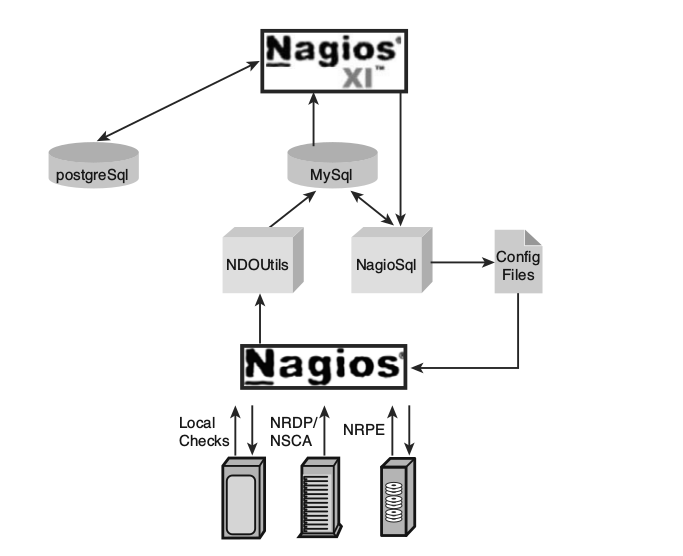
\includegraphics[width=\linewidth]{images/nagios-architecture}}
\caption{Nagios Architecture}
\label{fig:nagios-architecture}
\end{figure}



\section{Conclusion}
Put in some conclusion based on what you have researched.  Use cases,
educational materials can be added to this.  In addition to that ways
Nagios can be improved to get better performance can be included in
your conclusion. With the Gitlab incidence, we can see how
untrustworthy the machines can be. This is also why we need Nagios.



% Bibliography

\bibliography{references}
 
%\newpage

\appendix


\end{document}
